Convolutional networks, \cite{Deep Learning} also known as convolutional neural networks or CNN, are a specialized kind of artificial neural network for processing data that has a known, grid-like topology. Examples include time-series data, which can be thought of as a 1D grid taking samples at regular time intervals, and image data, which can be thought of as a 2D grid of pixels. Convolutional networks are simply neural networks that use convolution in place of general matrix multiplication in at least one of their layers.\\

The main strengths of CNNs are to provide an efficient dense network which performs the prediction or identification etc. efficiently. CNNs are the most popular topic in the pool of deep learning, which is indeed very vast, and this is usually because of the ConvNets. Immense datasets are applied to CNNs, it is even considered that larger the data, greater the accuracy will result, otherwise other operations such as transfer learning shall be applied to expand the data. The power of CNN is to detect distinct features from images all by itself, without any actual human intervention.\\

There are multiple benefits of using this model as the state of art neural network. As it can be used in various fields and perform major tasks like facial recognition, analyzing documents, understanding climate, and image recognition and object identification etc. Deep learning has helped enormously in advancement of the science fields and CNN is the most popular one as it attains the benefits of providing maximum performance and efficiency.\\

Traditional neural network layers use matrix multiplication by a matrix of
parameters with a separate parameter describing the interaction between each input
unit and each output unit. This means every output unit interacts with every input
unit. Convolutional networks, however, typically have sparse interactions (also
referred to as sparse connectivity or sparse weights). This is accomplished by
making the kernel smaller than the input. For example, when processing an image,
the input image might have thousands or millions of pixels, but we can detect small,
meaningful features such as edges with kernels that occupy only tens or hundreds of
pixels. This means that we need to store fewer parameters, which both reduces the
memory requirements of the model and improves its statistical efficiency. It also
means that computing the output requires fewer operations. These improvements
in efficiency are usually quite large. If there are m inputs and n outputs, then
matrix multiplication requires m x n parameters and the algorithms used in practice
have O(m x n) run-time. If we limit the number of connections
each output may have to k, then the sparsely connected approach requires only
k x n parameters and O(k x n) run-time. For many practical applications, it is
possible to obtain good performance on the machine learning task while keeping
k several orders of magnitude smaller than m. \\


Each convolutional layer contains a series of filters known as convolutional kernels. The filter is a matrix of integers that are used on a subset of the input pixel values, the same size as the kernel. Each pixel is multiplied by the corresponding value in the kernel, then the result is summed up for a single value for simplicity representing a grid cell, like a pixel, in the output channel/feature map. In computer vision the input is often a 3 channel RGB image. For simplicity, if we take a grey-scale image that has one channel (a two dimensional matrix) and a 3x3 convolutional kernel (a two dimensional matrix). The kernel strides over the input matrix of numbers moving horizontally column by column, sliding/scanning over the first rows in the matrix containing the images pixel values. Then the kernel strides down vertically to subsequent rows. Note, the filter may stride over one or several pixels at a time, this is detailed further below.


 \begin{figure}[h]
	\centering
	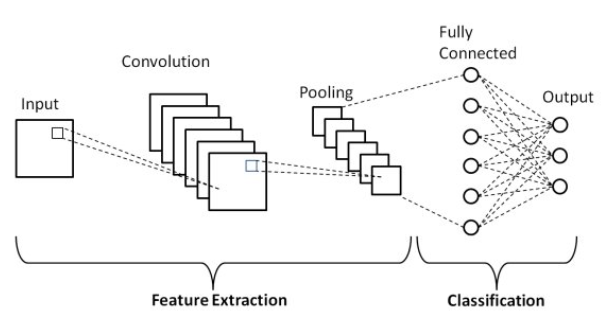
\includegraphics[width=0.8\textwidth]{figures/background/CNN.png}
	\captionsetup{labelformat=empty}
	\caption{\href{https://www.researchgate.net/publication/336805909/figure/fig1/AS:817888827023360@1572011300751/Schematic-diagram-of-a-basic-convolutional-neural-network-CNN-architecture-26.ppm}
	{Basic Convolution Neural Network Architecture}}
\end{figure}

\pagebreak